% Preamble
\documentclass[14pt]{article}
%encoding
%--------------------------------------
\usepackage[T1]{fontenc}
\usepackage[utf8]{inputenc}
\usepackage[portuguese]{babel}
\usepackage{hyphenat}
\usepackage{fancyhdr}
\usepackage{graphicx}
\usepackage{float}
\usepackage{geometry}
\usepackage{hyperref}

\geometry{
a4paper,
total={170mm,257mm},
left=20mm,
top=20mm,
}

\hyphenation{mate-mática recu-perar}


\pagestyle{fancy}
\fancyhf{}
\fancyhead[LE,RO]{AED}
\fancyhead[RE,LO]{AirRoutes}
\fancyfoot[RE,CO]{António Vidais \and Tiago Leite}
\fancyfoot[LE,RO]{\thepage}
\graphicspath{ {images/} }
%--------------------------------------
\title{AirRoutes - Algoritmos e Estruturas de Dados}
\date{Dezembro de 2020}
\author{António Vidais \\96162 \and Tiago Leite \\96332}
% Document
\begin{document}
    \maketitle

    \section{Descrição do Problema} \label{sec:d.problema}
    Este projeto, criado no âmbito da Unidade Curricular de Algoritmos e Estruturas de Dados, aborda o problema de
    encontrar um conjunto mínimo de rotas que garantam a existência de um caminho entre cada par de aeroportos,
    sem qualquer redundância.
    O Programa que este projeto visa produzir deve não só produzir uma rede mínima de rotas, mas sim a rede que garante
    todos os destinos já existentes, com o menor custo.
    Uma ferramenta como esta pode ser necessária, em termos práticos,quando uma companhia aérea se encontra num cenário
    de contenção de custos.
    Numa situação desta natureza, poderá ser necessário reduzir o seu conjunto de rotas à rede que
    garante que todos os aeroportos nela podem ser utilizados, com o menor custo.

    O Projeto que este relatório descreve foi desenvolvido na linguagem C e, para o seu correto funcionamento deve
    receber as informações de todas as rotas existentes através de um ficheiro de texto.
    Este deve conter uma ou mais redes de aeroportos, cada uma devidamente identificada com um cabeçalho contendo o
    número de aeroportos, o número total de rotas existentes e a variante que se pertende obter.
    Terminada a execução, o programa produz um segundo ficheiro de texto que contêm o conjunto mínimo de menor custo
    para cada rede fornecida, também identificados pelo cabeçalho fornecido, com a adição de algumas informações úteis,
    como o número de rotas mantidas e o custo total da rede

    \section{Abordagem do Problema}\label{sec:abordagem.problema}
    Para resolver este problema, foi necessário criar uma estrutura capaz de guardar uma representação do grafo formado
    pelo conjunto de rotas fornecido.
    A escolha desta estrutura requer uma análise cuidada ao tipo de grafo (denso ou esparço)e aos algoritmos que se
    pretende utilizar.
    Uma má escolha poderia levar a tempos de execução muito maiores que os pretendidos e maior utilização de memória,
    devido ao aumento da complexidade.

    \section{Arquitetura do Projeto}\label{arquitetura.projeto}
    A estrutura geral do programa é apresentada na Figura \ref{fig:main.flowchart}.
    Após verificar e inicializar os ficheiros necessários, procede-se à leitura dos Argumentos.
    Dependendo da leitura dos argumentos, é decidida a melhor forma de representação do grafo para o problema
    em questâo.
    As formas de representação do grafo são definidas com maior detalhe na secção\ref{sec:formas.representar.grafo}.

    \begin{figure}[H]
        \centering
        \label{fig:main.flowchart}
        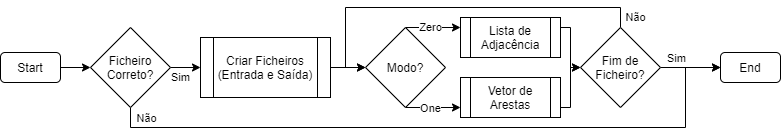
\includegraphics[scale=0.45]{main.flowchart.png}
        \caption{Fluxograma Representativo da execução da função main}
    \end{figure}

    \newpage

    \section{Estruturas e Tipos de Dados}\label{sec:estruturas.tipos.dados}

    \subsection[PBArg]{Argumentos do Problema}\label{subsec:argumentos.problema}
    A estrutura do tipo PBArg é usada para guardar os argumentos do problema. È declarada no ficheiro \emph{Graph.h}.
    Esta Estrutura é composta por:
    \begin{itemize}
        \item v : Integer que guarda o número de vértices no grafo;
        \item e : Integer que guarda o número de arestas no grafo;
        \item vi : Integer que guarda o 1º vértice da aresta a eliminar, nos modos aplicáveis;
        \item vj : Integer que guarda o 2º vértice da aresta a eliminar, nos modos aplicáveis;
        \item var : String que guarda a variante do problema pretendida;
        \item err : Boolean que é ativada quando ocorrem erros durante a execução;
    \end{itemize}

    \subsection[edge]{Aresta}\label{subsec:aresta}
    A estrutura do tipo Aresta é usada para guardar uma aresta, quer durante a sua leitura em ambos os modos, quer na
    sua manipulação no modo 1, onde está inserida na estrutura graph, para formar o vetor de arestas. Apesar de
    relativamente simples, esta estrutura é a base sobre a qual a maioria das funções deste programa operam. Por esse
    motivo foi propositamente tornada mais simples e eficiente.
    Esta Estrutura é composta por:
    \begin{itemize}
        \item vi : Integer que guarda o 1º Vértice da Aresta
        \item vj : Integer que guarda o 2º Vértice da Aresta
        \item cost : double que guarda o custo da aresta
    \end{itemize}

    \subsection[list]{Lista de Adjacências}\label{subsec:l.adj}
    A estrutura do tipo Lista de Adjacências é utilizada pelas funções do modo 0.
    Esta é a base para a representação do grafo sob a forma de vetor de listas de adjacências.
    As razões pelas quais esta representação do grafo foi escolhida para o modo 0 será discutida n\ref{subsec:formas.represent.grafo}.
    Esta Estrutura é composta por:
    \begin{itemize}
        \item v : Integer que guarda o vértice base da lista, a partir do qual se encontram os adjacentes;
        \item cost : Double que guarda o custo da aresta entra o vértice e o 1º vértice adjacente;
        \item next : Apontador para list que guarda o próximo elemento da lista;
    \end{itemize}

    \subsection[graph0]{Grafo sob a forma de Lista de Adjacência}\label{subsec:grafo.l.adj}
    A estrutura do tipo graph0 é a estrutura mãe para a representação do grafo na forma de listas de adjacências.
    Decidiu-se anexar à representação propriamente dita um apontador para \nameref{subsec:argumentos.problema} para
    facilitar grande parte dos parâmetros de entrada das funções.
    Assim, os \ref{subsec:argumentos.problema} são enviados em conjunto com a representação do grafo.
    Esta Estrutura é composta por:
    \begin{itemize}
        \item Arg : Estrutura do tipo \nameref{subsec:argumentos.problema} que guarda os argumentos referentes ao grafo
        representado no outro membro desta estrutura;
        \item data : Vetor de estruturas do tipo \nameref{subsec:l.adj} que guarda a lista de adjacências de todos os
        vértices do grafo;
    \end{itemize}

    \subsection[graph]{Grafo sob a forma de Vetor de Arestas}\label{subsec:grafo.v.are}
    A estrutura do tipo graph é a estrutura mãe da representação do grafo na forma de vetor de arestas.
    Como a estrutura \nameref{subsec:grafo.l.adj}, a estrutura \nameref{subsec:grafo.v.are} inclui um apontador para uma estrutura
    do tipo \nameref{subsec:argumentos.problema} para facilitar os parâmetros de entrada de grande parte das funções que operam
    sobre o grafo.
    Esta Estrutura é composta por:
    \begin{itemize}
        \item Arg : Estrutura do tipo \nameref{subsec:argumentos.problema} que guarda os argumentos referentes ao grafo apontado pelo vetor de arestas;
        \item data : Vetor de estruturas do tipo \nameref{subsec:aresta} que guarda todas as arestas lidas do ficheiro de entrada para o grafo em estudo;
    \end{itemize}

\end{document}